% This text is a supplement of CINTA.
% May. 2018
% Author: Libin Wang
% SCNU
% additional use of \usepackage{beamerthemesplit}
\documentclass{beamer}

%%%%%%%%%%%%%%%%%%%%%%%%%%%%%%%%%%%%%%%%%%%%%%%%%%%%%%%%%%%%%%%%%%%%%
\usepackage{xeCJK}
%\usepackage[CJKbookmarks]{hyperref}

%% Support Chinese with TeX Live fonts.

\setCJKmainfont[
  BoldFont=FandolHei-Regular.otf,
  ItalicFont=FandolKai-Regular.otf,
  BoldItalicFont=FandolKai-Regular.otf
]{FandolSong-Regular.otf}
\setCJKsansfont[AutoFakeBold, AutoFakeSlant]{FandolHei-Regular.otf}
\setCJKmonofont{FandolFang-Regular.otf}

\setmainfont{Times New Roman} % 设置默认英文衬线字体

\setCJKfamilyfont{ls}{FandolSong-Regular.otf} %定义字体
%%%%%%%%%%%%%%%%%%%%%%%%%%%%%%%%%%%%%%%%%%%%%%%%%%%%%%%%%%%%%%%%%%%%%

%\usepackage{beamerthemesplit} % new 
\usepackage{beamerthemeshadow}
\setbeamertemplate{headline}{}
\setbeamertemplate{footline}{}
\setbeamertemplate{navigation symbols}{}
\usepackage{amsmath, amsfonts, amssymb}

%% Setup for Code
\usepackage{listings}
\lstset{language = Python,
	showstringspaces = false,
	columns = fullflexible,
	numbers = left,
	numberstyle = \tiny,
	frame = single}

\newtheorem{proposition}[theorem]{Proposition}

%\title{A Concrete Introduction to Number Theory and Algebra--群、子群、循环群} 
\title{Mathematics for Computer Science -- Group, Subgroup and Cyclic Group} 
\author{Libin Wang} 
\institute{Shool of Computer Science, South China Normal University}
\date{\today} 

\begin{document}

\frame{\titlepage} 

\frame{\frametitle{Table of contents}\tableofcontents} 

\section{Group} 

\frame{\frametitle{提醒.} 

\begin{block}{提醒.}
以下群论内容不仅仅是开启了新的学习方向，而是对之前数论相关内容的重新审视和抽象，形成一次二重奏。而且，我们会从思考与抽象中得到更多的洞见，还有乐趣！
\end{block}
}

\frame{\frametitle{Motivation.} 

\begin{block}{抽象.}
抽象：发现已知的世界中事物的共性与区别，忽略掉某些细节，得到一种更通用、更宽泛、可以描述更广阔世界的框架或语言，从而探求未知世界的知识。

\end{block}
\pause

\begin{alertblock}{Question.}
更给出（或找出）更适合你自己的“抽象”的定义。
\end{alertblock}
}
\frame{\frametitle{Motivation.} 

\begin{block}{重新审视“消去律”.}
In last chapter, we extremely rely on \textit{Cancellation Law}. 

If $\gcd(c, m) = 1$ and $ac \equiv bc \pmod{m}$, then
\[
a \equiv b \pmod{m}.
\]
\end{block}
\pause

\begin{alertblock}{Question.}
	Actually, what is cancellation?
\end{alertblock}
}

\frame{\frametitle{Motivation.} 
\begin{block}{Ideas.}
	From $ac \equiv bc \pmod{m}$ to $a \equiv b \pmod{m}$, seemingly, we need division, actually we need multiplication:
	
	\[
	acc^{-1} \equiv bcc^{-1}\pmod{m}.
	\]
	
	Hence by $cc^{-1} \equiv 1\pmod{m}$, we have 
	
	\[
	a \equiv b \pmod{m}.
	\]
	
	Why $c^{-1}$ exists? Because of $\gcd(c,m)=1$!
	
\end{block}
	
}

\frame{\frametitle{Motivation.} 
	\begin{block}{Additional conditions.}
	Need more conditions?\pause
	
	Yes, we need \emph{associativity}:
	\[
	(ac)c^{-1} \equiv a(cc^{-1})\pmod{m},
	\]
	
	and \emph{closure}, which means that we only consider numbers from a specified set.
   \end{block}
	\pause
	\begin{alertblock}{Question.}
		什么数学操作不满足结合律?
	\end{alertblock}
}

\frame{\frametitle{Motivation.} 
	\begin{block}{Wrap up.}
       Wrap these up. For  a set $\mathbb{G}$ and an operator $\cdot$  on the elements, we need:
\begin{itemize}
	\item \emph{Closure}: $\forall a,b \in \mathbb{G}, \quad a\cdot b \in \mathbb{G}$.
	
	\item \emph{Associativity}: $(a\cdot b)\cdot c = a\cdot (b\cdot c)$.
	
	\item An element "$1$" called  \emph{identity}, such that $1\cdot a = a \cdot 1 = a$.
	
	\item $\forall a\in \mathbb{G}$, there exists $a^{-1}\in \mathbb{G}$, such that $a\cdot a^{-1} = 1 = a^{-1} a$, called \emph{inverse}.

\end{itemize}

\end{block}
}

\frame{\frametitle{Group（群）.} 
	
	\begin{block}{Definition of Group.}
		A group is a set $\mathbb{G}$ together with an operation $\cdot$ satisfying the following axioms:
	 
	\begin{itemize}
		\item \emph{Closure(封闭性)}: $\forall a,b \in \mathbb{G}, \quad a\cdot b \in \mathbb{G}$.
		
		\item \emph{Associativity(结合律)}: $(a\cdot b)\cdot c = a\cdot (b\cdot c)$.
		
		\item There is an element $e\in \mathbb{G}$, called \emph{identity(单位元)}, such that $e\cdot a = a \cdot e = a$.
		
		\item $\forall a\in \mathbb{G}$, there exists $a^{-1}\in \mathbb{G}$, called \emph{inverse(逆元)}, such that $a\cdot a^{-1} = e = a^{-1} \cdot a$.
	\end{itemize}
\end{block}
	
}

\frame{\frametitle{Examples of groups.} 
	\begin{exampleblock}{Groups.}
		\begin{itemize}
           \item $(\mathbb{Z}, +)$ is a group, while $(\mathbb{Z}, \times)$ is not a group.
           \item $(\mathbb{Q}, +)$ and $(\mathbb{R}, +)$ are groups.
	       \item $(\mathbb{Q}^*, \times)$ and $(\mathbb{R}^*, \times)$ are groups.
	    \end{itemize}
	\end{exampleblock}\pause
\begin{alertblock}{Check.}
	Please check and know why.
\end{alertblock}
}

\frame{\frametitle{Examples of some important groups.} 
\begin{exampleblock}{$\mathbb{Z}_n$}
Let $n$ be an integer, the set $\mathbb{Z}_n = \{0, 1, 2, \cdots, n-1\}$ forms a group under the operation of addition. However, $(\mathbb{Z}_n, \times)$ is not a group.
\end{exampleblock}\pause

\begin{exampleblock}{$\mathbb{Z}_p^*$}
	Let $p$ be a prime number, the set $\mathbb{Z}_p^* = \{1, 2, \cdots, p-1\}$ forms a group under the operation of multiplication. (Recall Fermat's Little Theorem.)
\end{exampleblock}\pause

\begin{exampleblock}{$\mathbb{Z}_n^*$}
	Let $n$ be an integer, the set $\mathbb{Z}_n^* = \{a \in \mathbb{Z}_n: \gcd(a,n)=1\}$ forms a group under the operation of multiplication. (Recall Euler's Theorem.)
\end{exampleblock}
}

\frame{\frametitle{An important group: nth root of unity.} 
\begin{example}%{$\mathbb{U}_n}
	\label{exm:nth_root_of_unity}
	设$n$为正整数，称方程$z^n = 1$在复数上的所有解为$n$次单位根，记为$\mathbb{U}_n = \{z \in \mathbb{C}:  z^n = 1\} $。
	根据高等数学相关知识可知，$\mathbb{U}_n = \{e^{\frac{2\pi i k}{n}}, k = 0, 1, \cdots , n - 1\}$，并且
	\[ e^{\frac{2\pi i k}{n}} = \cos(\frac{2 \pi k}{n}) + i \sin(\frac{2\pi k}{n}), k = 0, 1, \cdots , n - 1\]
	如果记$\omega = \cos(\frac{2 \pi }{n}) + i \sin(\frac{2\pi }{n})$，则可更简洁地表示$n$次单位根为
	\[\mathbb{U}_n = \{\omega^i, i = 0, 1, \cdots , n - 1\}\]
	可证明$\mathbb{U}_n $ 在复数的乘法上形成群(这是课后习题)，并称$\mathbb{U}_n $ 为$n$次\emph{单位根群}。
\end{example}
}

\frame{\frametitle{8th root of unity.} 
\begin{figure}
	\begin{center}
		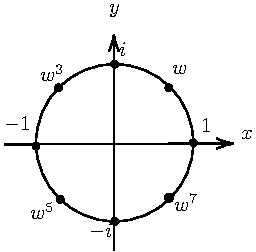
\includegraphics[scale=1.5]{../figures/nth-unity.pdf} 	
		\caption{$8$次单位根群}
		\label{fig:nth_root_unity}       % Give a unique label
	\end{center}
\end{figure}
}

\frame{\frametitle{思考} 

	\begin{alertblock}{Thinking.}
		$\mathbb{Z}_n$ 与$\mathbb{U}_n$ 的操作行为很类似吗？这会意味什么呢？
		另外，$\mathbb{U}_n$ 的操作行为与$\mathbb{Z}_p^*$不很类似，是吗？
	\end{alertblock}
}


%----------------------------
%第二章
%----------------------------

\section{Basic Properties of Groups} 
\label{sec:prop_gr}

\frame{\frametitle{Basic Properties of Groups.}
\begin{proposition}[Proposition 1.]
	The identity element in a group $\mathbb{G}$ is unique; that is, there exists only one element $e \in \mathbb{G}$ such that $eg= ge = g$ for all $g\in \mathbb{G}$.
\end{proposition}

\pause

\begin{proof}
	Suppose $\exists e, e' \in \mathbb{G}$ are identities. Then：
	\begin{itemize}
		\item $e e' = e'$
		
		\item $e e' = e$
	\end{itemize}
    Combining these two equations, we have $e = e e' = e'$.
\end{proof}
}

\frame{\frametitle{Proposition 2.}
	\begin{proposition}[Proposition 2.]
		If $\forall g \in \mathbb{G}$, then the inverse of $g$, $g^{-1}$, is unique.
	\end{proposition}
	\begin{proof}
			如果$g^{-1}$和$g'$都是$g$的逆元，则有
			\[ g' = g' e = g' (g g^{-1}) = (g' g)g^{-1} = e g^{-1} = g^{-1}.\]
	\end{proof}
}

\frame{\frametitle{Proposition 3.}
	
	\begin{proposition}[Proposition 3.]
		Let $\mathbb{G}$ be a group. If $a, b \in \mathbb{G}$, then $(ab)^{-1} = b^{-1} a^{-1}$.
	\end{proposition}

	\begin{proof}
		By construction.
		\begin{itemize}
			\item $ab(b^{-1}a^{-1}) = e$.
			
			\item $(b^{-1}a^{-1}) a b = e$.
		\end{itemize}
		Combining these two equations, we know, the inverse of $(ab)$ is $b^{-1}a^{-1}$.
	\end{proof}
}

\frame{\frametitle{Proposition 4.}
	\begin{proposition}[Proposition 4.]
		Let $\mathbb{G}$ be a group, $\forall g \in \mathbb{G}$, $(g^{-1})^{-1} = g$.
	\end{proposition}
	
	\pause

	\begin{proof}
	By definition,	$g g^{-1}=e$ and $g^{-1}(g^{-1})^{-1} = e$. Hence:
				\[
				(g^{-1})^{-1} = (g g^{-1}) (g^{-1})^{-1} = g( g^{-1} (g^{-1})^{-1})= ge = g .
				\]
	\end{proof}
	\pause
	\begin{alertblock}{另一种思路.}
	该命题要证明的是$g^{-1}$的逆元是$g$。根据$g^{-1}$的定义，“交换”$g$与$g^{-1}$的位置，即得！
	\end{alertblock}
}

\frame{\frametitle{Proposition 5.}
	\begin{proposition}[Proposition 5.]
		Let $\mathbb{G}$ be a group. For any $a, b \in \mathbb{G}$. Then each of the equations $ax = b$ and $xa = b$ has a unique solution in $\mathbb{G}$.
	\end{proposition}
	
	\pause
	
	\begin{proof}
		\begin{itemize}
			\item Existence. Such an $x$ exists.
			
			\item Uniqueness. Suppose that $x_1$ and $x_2$ are both solutions $\ldots$
		\end{itemize}
	Left as an exercise.
	\end{proof}
}

\frame{\frametitle{Proposition 6.}
	\begin{proposition}[Cancellation Law.]
		Let $\mathbb{G}$ be a group, and $a, b, c \in \mathbb{G}$. Then $ba = ca$ implies $b = c$ and $ab = ac$ implies $b = c$.
	\end{proposition}
	
	\pause
	
	\begin{proof}
		 Left as an exercise.
	\end{proof}\pause

\begin{alertblock}{A little thought.}
   Where does "\emph{Cancellation Law}" come from?
\end{alertblock}
}

\frame{\frametitle{思考一.}
\begin{exampleblock}{置换与消去律}
在费尔马小定理和欧拉定理的证明中，依赖消去律可得：

对任意素数$p$和与$p$互素的正整数$a$，$\mathbb{Z}_p^* =a \mathbb{Z}_p^* = \{ a i : \forall i \in \mathbb{Z}_p^* \}$; 

对任意合数$n$和与$n$互素的正整数$a$，$a \mathbb{Z}_n^* = \mathbb{Z}_n^*$。

请问，对任意的群$\mathbb{G}$和群元$a$，
是否有$ \mathbb{G} = a \mathbb{G} = \{a g : \forall g \in \mathbb{G} \} $？为什么？
\end{exampleblock}

}

\frame{\frametitle{思考二.}
	\begin{exampleblock}{逆元的唯一性源自什么？}
		回忆，模$n$的乘法逆元源自Bezout定理，然后我们分析过为什么乘法逆元唯一。
		请问，对任意的群$\mathbb{G}$，我们也有“逆元唯一”的结论，此时，逆元唯一源自于什么？
		这样的思考能给我们什么启发？
	\end{exampleblock}
	
}

\frame{\frametitle{课堂习题} 
	\begin{block}{课堂练习-1.}
	\label{ex:class-1}
		设$a$和$b$是群$\mathbb{G}$中的元素。如果$a^4 b = ba$且$a^3 = e$，证明$ab= ba$。
	\end{block}
		
	\begin{block}{课堂练习-2.}
	\label{ex:class-2}
		设$a$和$b$是群$\mathbb{G}$中的元素。证明，对任意$n\in \mathbb{Z}$，有$a b^n a^{-1} = (aba^{-1})^n$。
	\end{block}
}

\frame{\frametitle{Notations.}
Let $\mathbb{G}$ be a group, and $g \in \mathbb{G}$. For $n\in \mathbb{N}$. 
	\begin{block}{Notations.}
       \begin{itemize}
       	\item $g^0 = e$
       	\item $g^n = \underbrace{g\cdot g \cdots g}_{\text{n times}}$
       	\item $g^{-n} = \underbrace{g^{-1}\cdot g^{-1} \cdots g^{-1}}_{\text{n times}}$
       \end{itemize}
    \end{block}

	\begin{block}{Order.}
       The order of a finite group is the number of elements that it contains. If $\mathbb{G}$ is a group containing $n$ elements, we write $\vert \mathbb{G} \vert = n$. 
   \end{block}

}

\section{Subgroups}

\frame{\frametitle{Definitions}
\begin{definition}{(Subgroup.)（子群）}
	
	Let $\mathbb{G}$ be a group and $\mathbb{H}$ a subset of $\mathbb{G}$. If $\mathbb{H}$ is a group under group operation in $\mathbb{G}$, then $\mathbb{H}$
	is said to be a subgroup of $\mathbb{G}$, denoted by $\mathbb{H}\leq \mathbb{G}$.

\end{definition}

}

\frame{\frametitle{Examples of Subgroup.}
	\begin{exampleblock}{Examples of Subgroup.}
          \begin{itemize}
          	 \item For any group $\mathbb{G}$, there is a trivial subgroup $\{ e \}$.
          	 
          	 \item The additive groups: $\mathbb{Z} \leq \mathbb{Q} \leq \mathbb{R} \leq \mathbb{C}$.
          	 
          	 \item $\forall n \in \mathbb{Z}$, $n\mathbb{Z} = \{ kn | k \in \mathbb{Z}\}$ is a subgroup of $\mathbb{Z}$.
          \end{itemize}
	\end{exampleblock}
}

\frame{\frametitle{Examples of Subgroup.}
	\begin{exampleblock}{ Subgroup of $\mathbb{Z}_p^*$.}
	Let $p$ be a prime, for all $i \in \mathbb{Z}_p^*$, compute $i^2 \bmod{p}$, form a set $\mathbb{S} = \{ i^2 \bmod{p}, \forall i \in \mathbb{Z}_p^*\}$. Check that $\mathbb{S}$ is a group under the operation of multiplication, namely $\mathbb{S}$ is a subgroup of $\mathbb{Z}_p^*$. What is the order of $\mathbb{S}$?
	\end{exampleblock}
}	

\frame{\frametitle{Properties of Subgroup.}
	\begin{exampleblock}{Exercise.}
		Write a program to play with $\mathbb{Z}_n^*$.
		\begin{itemize}
			\item Given an integer $n$, construct the multiplicative group $\mathbb{Z}_n^*$;
			
			\item Find a subgroup of the group $\mathbb{Z}_n^*$;
			
			\item Find a relation between the size of subgroup and the size of $\mathbb{Z}_n^*$.
		\end{itemize}
	\end{exampleblock}
}

\frame{\frametitle{Properties of subgroup.}
	\begin{proposition}[(Subgroup.)]
		A nonempty subset $\mathbb{H}$ of a group $\mathbb{G}$  is a subgroup of  $\mathbb{G}$ if and only if $\mathbb{H} \neq \emptyset$, and $ab^{-1} \in \mathbb{H}$ for all $a, b \in \mathbb{H}$.
	\end{proposition}

\begin{proof}
	Two directions. The $\rightarrow$ part is easy. For $\leftarrow$ part, you need to check that $\mathbb{H}$ satisfies all the axioms of a group.
\end{proof}
}

\frame{\frametitle{子群判定方法.}
\begin{exampleblock}{有多少种判定子群的方法？}
给定群$\mathbb{G}$和其子集$\mathbb{H}$，如何判断$\mathbb{H}$是否$\mathbb{G}$的子群？
\begin{itemize}
\item 验证四条群公理.

\item 命题6.8：封闭性、有逆元.

\item 命题6.9：$\mathbb{H} \neq \emptyset$, and $ab^{-1} \in \mathbb{H}$ for all $a, b \in \mathbb{H}$.

\item 命题6.10：针对有限群，只需要验证封闭性.
\end{itemize}
\end{exampleblock}
}

\frame{\frametitle{子群判断.}
	\begin{exampleblock}{练习题.}

		\begin{itemize}
			\item 证明：任意群$\mathbb{G}$的两个子群的交集也是群$\mathbb{G}$的子群。
			
			\item 证明或证伪：任意群$\mathbb{G}$的两个子群的并集也是群$\mathbb{G}$的子群。
			
			\item $\mathbb{G}$是阿贝尔群，$\mathbb{H}$和 $\mathbb{K}$是$\mathbb{G}$的子群。
			请证明$\mathbb{H} \mathbb{K} = \{hk: h \in \mathbb{H}, k \in \mathbb{K}\}$是群$\mathbb{G}$的子群。
			如果$\mathbb{G}$不是阿贝尔群，结论是否依然成立？
			
			\item 设$\mathbb{G}$是阿贝尔群，$m$是任意整数，记$\mathbb{G}^m = \{ g^m: g\in \mathbb{G}\}$。请证明$\mathbb{G}^m$是
			$\mathbb{G}$的一个子群。
			
			\item 设$\mathbb{G}$是阿贝尔群，$m$是任意整数，记$\mathbb{G}[m] = \{ g\in \mathbb{G}: g^m = e \}$。请证明$\mathbb{G}[m]$是
			$\mathbb{G}$的一个子群。 % 以上两题出自Shoup的NTA, P.133
		\end{itemize}
	\end{exampleblock}
}

\frame{\frametitle{习题.}
	\begin{exampleblock}{证明题.}
		证明：阿贝尔群$\mathbb{G}$中的有限阶元素形成子群。该子群有一个特殊的名字，称为\emph{挠子群}（\emph{Torsion Subgroup}）。
	\end{exampleblock}
	
}%20250320

\frame{\frametitle{课堂习题} 
	\begin{block}{课堂练习.}
		\label{ex:ex1}
		证明：对任意的$n \in \mathbb{Z}$，$n \mathbb{Z}$是$\mathbb{Z}$的子群，且$\mathbb{Z}$中的任意子群只能是某个$n \mathbb{Z}$。
	\end{block}
}

\section{Cyclic Groups}

\frame{\frametitle{Cyclic Groups（循环群）.}
	\begin{exampleblock}{Example of cyclic group.}
		Consider the following computation:
		Choose a number $g$ from $\mathbb{Z}_p^*$ randomly, $p$ is a prime, and compute:
		\[
		\mathbb{S} = \{ g, g^2, g^3, \cdots, g^i, \cdots \}
		\]
		\pause
		Questions:
		\begin{itemize}
			\item May $\mathbb{S}$ be finite? 
					
			\item May $\mathbb{S}$ be a group? Why or why not?
					
			\item Can $\mathbb{S}$  equals $\mathbb{Z}_p^*$?
		\end{itemize}
	\end{exampleblock}
}

\frame{\frametitle{Cyclic Groups.}
	\begin{exampleblock}{Example of cyclic group.}
		For example:
		For $p = 11$, choose $g = 4$, and compute:
		\[
		\mathbb{S} = \{ 4, 4^2, 4^3, \cdots, 4^i, \cdots \}
		\]
		\pause
		We will have:
		\[
		\mathbb{S} = \{ 4, 5, 9, 3, 1\}
		\]
		Certainly, it is finite and it is a group.\pause
		Questions:
		\begin{itemize}
			\item What will we get if $g = 2$? 
			
			\item What will we get if $g = 3$? 			
		\end{itemize}
	\end{exampleblock}
}

\frame{\frametitle{Cyclic Groups.}
	\begin{theorem}
		Let $\mathbb{G}$ be a group and $g$ be any element in $\mathbb{G}$. Then the set
			\[
			\langle g \rangle = \{ g^k: k \in \mathbb{Z} \}
			\]
	    is a subgroup of $\mathbb{G}$.  We call $\langle g \rangle$ the cyclic group generated by $g$, and $g$ is a generator of the group.
	\end{theorem}

	    \begin{proof}
	       Check the axioms.
       \end{proof}
}

\frame{\frametitle{Examples of Cyclic groups.} 
	\begin{exampleblock}{Some cyclic groups.}
		\begin{itemize}
           \item $(\mathbb{Z}, +)$ is a cyclic group, while $1$ is the generator.
        
	       \item $(\mathbb{Z}_n, +)$ is a cyclic group, while $1$ is the generator.
	       
	       \item $\langle i \rangle$ is a cyclic group, while $i$ is the generator.
	    \end{itemize}
	\end{exampleblock}\pause
\begin{alertblock}{Check.}
	Please check and know why.
\end{alertblock}
}

\frame{\frametitle{Examples of Cyclic groups.} 
	\begin{exampleblock}{Some cyclic groups.}
		\begin{itemize}
           \item ${Z}_p^*$ is a cyclic group, while $p$ is a prime.
        
	       \item $\mathbb{Z}_n^*$ is \emph{NOT} necessarily a cyclic group, while $n$ is composite.
	    \end{itemize}
	\end{exampleblock}\pause
\begin{alertblock}{Check.}
	Please check and know why.
\end{alertblock}
}

\frame{\frametitle{习题} 
	
	\begin{exampleblock}{单位根群.}
		$\mathbb{U}_n$ 是循环群吗？为什么，或者为什么不？
	\end{exampleblock}
}

\frame{\frametitle{Primitive Root（原根）}
\begin{definition}
Let $a$ and $n$ be relatively prime integers with $n>0$. The order of $a$ modulo $n$ is the smallest exponent $e \geq 1$ such that $a^e \equiv 1 \pmod{n}$. If the order of $a$ modulo $n$ equals the largest possible order modulo $n$, then $a$ is called a primitive root modulo $n$.
\end{definition}
}

\frame{\frametitle{Primitive Root}
\begin{exampleblock}{原根}
From the last example, we know the order of $4$ modulo $11$ is $5$, and the order of $2$ and $6$ modulo $11$ is $10$. Since the largest possible order modulo $11$ is $10$, 
thus $2$ and $6$ are two primitive roots modulo $11$. Using language of group, we may say that $\mathbb{Z}_{11}^*$ is a cyclic group generated by $2$ or $6$, 
and $2$ and $6$ are generators of $\mathbb{Z}_{11}^*$.
\end{exampleblock}
}

\frame{\frametitle{Properties of Cyclic Groups.}
\begin{proposition}
	%\label{prop:cyc_abel}
	所有的循环群都是阿贝尔群。
\end{proposition}

\begin{proposition}
	%\label{prop:sub_cyc}
	循环群$\mathbb{G}=\langle g \rangle$的每一个子群都是循环群。
\end{proposition}

}

\frame{\frametitle{Properties of Cyclic Groups.}
	\begin{theorem}
		Let $\mathbb{G} = \langle g \rangle$ be a cyclic group of order $n$. Then $g^k = e$ if and only if $n$ divides $k$.		
	\end{theorem}
\pause
	\begin{proof}
	Note that, $n$ is the least positive number such that $g^n = e$.\pause
	
	1. The $\leftarrow$ part is trivial, since $g^k = g^{ns} = e$. \pause
	
	2. The $\rightarrow$ part. 	Suppose $g^k = e$. By division algorithm, $k = nq +r$, where $0 \leq r < n$. Hence,
	\[
	e = g^k = g^{nq+r} = g^{nq} g^r = g^r.
	\]
	Thus, $r = 0$.
    \end{proof}
}

\frame{\frametitle{Properties of Cyclic Groups.}
	\begin{theorem}
		Let $\mathbb{G} = \langle g \rangle$ be a cyclic group of order $n$. If $h = g^k$ then the order of $h$ is $n/d$, where $d=\gcd(k,n)$.
	\end{theorem}
	\pause
	\begin{proof}
		Let $m$ be the least positive number such that $h^m = g^{km} = e$. \pause
		
		1. Then $n \mid km$, equivalently, $(n/d) \mid (k/d)m$. \pause
		
		2. Since $d = \gcd(k,n)$, $n/d$ and $k/d$ are relatively prime. Thus, $(n/d) \mid (k/d)m$ implies $(n/d) \mid m$. The smallest such $m$ is $n/d$.
	\end{proof}
}

\frame{\frametitle{Properties of Cyclic Groups.}
强调！
\begin{block}{循环群元素的阶.}
	$n$阶循环群$\mathbb{G} = \langle g \rangle$中的元素$g^k$的阶为：
	\[ \text{ord}(g^k) = \dfrac{n}{\gcd(k,n)}\]
\end{block}
	
}
\frame{\frametitle{Properties of Cyclic Groups.}
\begin{exampleblock}{通过生成元找生成元}
\label{exm:gen_gen}
	已知$2$是群$\mathbb{Z}_{11}^*$的生成元，群$\mathbb{Z}_{11}^*$的阶是$10$，$2^3 = 8 \in \mathbb{Z}_{11}^*$，且$\gcd(3, 10) =1$，所以
	$8$的阶是$10$，即$8$也是一个生成元。$5$不是生成元，因为$5 = 2^4 \bmod{11}$，$\gcd(4, 10) = 2$。请读者自行验证以上结论。
以上命题告诉我们，在知道某个元是生成元时，如何找到另一个生成元。
\end{exampleblock}
}

\frame{\frametitle{Properties of Cyclic Groups.}
\begin{exampleblock}{练习题.}
请找出群$\mathbb{Z}_{11}^*$的所有生成元。
\end{exampleblock}
}
%%% 20240509
\frame{\frametitle{Properties of Cyclic Groups.}
\begin{exampleblock}{思考题.}
已知$g$的阶为$n$，则$g^s$的阶$k$必然整除$n$。你能立即想到理由吗？
如果$n$为素数，那么任意$g^s$的阶会是什么？
\end{exampleblock}
% 从阶立即想到群，想到生成元.
}

\frame{\frametitle{Properties of Cyclic Groups.}
\begin{corollary}
		\label{cor:cyc_gr1}
			Let $\mathbb{G} = \langle g \rangle$ be a cyclic group of order $n$ then there are exactly $\varphi(n)$ generators in $\mathbb{G}$.
		\end{corollary}
		\pause
		
\begin{proof}
			There are $n$ elements in $\mathbb{G}$ with the form $g^i$, for all $i \in \mathbb{Z}_n$. For arbitrary $g^i$, its order is $n/d$, where $d = \gcd(i, n)$, then $g^i$ is a generator when $d = 1 $ which means $i$ is relatively prime to $n$. 
			There are $\varphi(n)$ elements
            in $\mathbb{Z}_n$ that are relatively prime to $n$, therefore there are $\varphi(n)$ generators in $\mathbb{G}$.
		\end{proof}
}

\frame{\frametitle{Properties of Cyclic Groups.}

\begin{corollary}
		\label{cor:cyc_gr2}
			Let $\mathbb{G} = \langle g \rangle$ be a cyclic group of order $p$, where $p$ is a prime,  then all elements in $\mathbb{G}$ except $e$ are generators.
\end{corollary}
		
		\begin{proof}
		Trivially from Corollary \ref{cor:cyc_gr1}.		
		\end{proof}
}

\frame{\frametitle{Properties of Cyclic Groups.}
	
	\begin{corollary}
		\label{cor:ord_div_n}
		%\label{cor:ord_div_n}
		设群$\mathbb{G} = \langle g \rangle$ 是阶为 $n$的循环群，则任意$h\in \mathbb{G} $的阶必整除$n$。
	\end{corollary}
	\begin{proof}
		该结论的正确性可直接由命题7.5得出。
	\end{proof}

}
\frame{\frametitle{Properties of Cyclic Groups.}
	以下是一种常见的思考方式，请大家注意。
	\begin{alertblock}{强调！}
	任意群中阶为$n$的元素$g$，可将群元素$g$的阶视为循环子群$\langle g \rangle$的阶:
		\[ \text{ord}(g) = |\langle g \rangle| = n.\]	
	\end{alertblock}
	
}

\frame{\frametitle{Properties of Cyclic Groups.}
	\begin{exampleblock}{Exercise-1.}
	\begin{itemize}
				\item 请心算列举出群$\mathbb{Z}_{10}$的所有生成元。
				
				\item 群$\mathbb{Z}_{17}^*$有多少个生成元？已知$3$是其中一个生成元，请问$9$和$10$是否生成元？%ans: 8, no, yes !
				
				\item $p$和$q$是两个不同的素数，请问$\mathbb{Z}_{pq}$都多少个生成元？$r$是任意正整数，请问$\mathbb{Z}_{p^r}$都多少个生成元？
				
				\item 请问$\mathbb{U}_n$中有多少个生成元，
				它们分别具有什么形式？
				
				\item 证明：如果$p$是素数，则加法群$\mathbb{Z}_p$没有非平凡真子群。
				
	\end{itemize}
	\end{exampleblock}
}

\frame{\frametitle{Properties of Cyclic Groups.}
	\begin{exampleblock}{Exercise.}
	\begin{itemize}
		       \item 证明：如果群$\mathbb{G}$是阶为$m$的循环群，且$d \mid m$，则
		       $\mathbb{G}$必有$d$阶子群。
		
				\item 证明：设$n$为正整数，对任意阶为$n$的循环群$\mathbb{G}$，如果存在整数$d$是$n$的因子，则群$\mathbb{G}$
				中存在$d$阶元素，且有$\varphi(d)$个$d$阶元素。%%% 20250326
				
				\item 设$n$是正整数，加法群$\mathbb{Z}_n$是一个循环群。你能否利用本章的知识来证明第四章最后一道习题呢？即：$\Sigma_{d|n}(\varphi(d)) = n$。
				
				
	\end{itemize}
	\end{exampleblock}
}

\frame{\frametitle{Properties of Cyclic Groups.}
	\begin{exampleblock}{Exercise.}
		\begin{itemize}
			\item 设$a$是任意群$\mathbb{G}$的元素。请问子群$\langle a^m \rangle \cap \langle b^n\rangle$的生成元是什么？
			
			
		\end{itemize}
	\end{exampleblock}
}

\frame{\frametitle{Primitive Root Theorem}
\begin{theorem}
\label{thm:primi_root}
{(Primitive Root Theorem.)} Every prime $p$ has a primitive root modulo $p$, and there are exactly $\varphi(p-1)$ primitive roots modulo $p$.
\end{theorem}
}

\frame{\frametitle{General Primitive Root Theorem}
\begin{theorem}
\label{thm:gen_primi_root}
The group $\mathbb{Z}_n^*$ is cyclic if and only if $n=2,4,p^e$, or $2p^e$, where $p$ is an odd prime and $e$ is a positive integer.
\end{theorem}
}

\frame{\frametitle{原根判定算法}
	\begin{block}{目标与思路.}
		\begin{itemize}
			\item 目标：输入$a$和$p$，判断$a$是模$p$的原根
			
			\item 算法基础：命题7.5展示，任意元素$a$的阶都是$p-1$（群阶）的因子；反之，只要$a$的阶不是小于$p-1$的因子，那么$a$的阶就是$p-1$，即为原根。
			
			\item 思路：排除法，对群阶的所有因子$d$进行判断，如果有$a^d \equiv  1 \pmod{p}$，则$a$不是原根。
			
			\item 实现过程：找出群阶的所有素因子，然后...
		\end{itemize}
	\end{block}
}

\frame{\frametitle{原根判定算法}
\begin{center}
	\lstinputlisting[label = alg:is_prim_rt, caption  = 原根判定算法]{../codes/is_prim_rt.py}
\end{center}
}

\frame{\frametitle{原根判定算法}
	\begin{block}{若干值得注意的问题.}
		\begin{itemize}
			\item 该算法的效率该如何衡量？该算法效率的瓶颈在哪里？
			
			\item 注意：排除法是枚举所有的因子；但是，算法第一步求的是$p-1$的素因子，不是求出所有因子。
			
			\item 算法中求所有素因子的函数如何用SageMath方便地实现？
		\end{itemize}
	\end{block}
}


\section{Coset and Lagrange's Theorem}

\frame{\frametitle{思考}
	\begin{block}{思考.}
		现在，有群、子群、循环群的概念，试图进一步考察群结构。群结构是目标，子群是研究群结构的基础，构造循环子群是找到子群的最直接方法。那么，我们接下来要做什么？
	\end{block}
}

\frame{\frametitle{Coset（陪集）}
	\begin{block}{Definition of Coset.}
		Let $\mathbb{G}$ be a group and $\mathbb{H}$ a subgroup of $\mathbb{G}$. Define a left coset of $\mathbb{H}$ with representative $g \in \mathbb{G}$ to be the set
		\[
		g\mathbb{H} = \{gh: h \in \mathbb{H}\}.
		\]
	    
	    Right coset can be defined similarly by
	    \[
	    \mathbb{H}g = \{hg: h \in \mathbb{H}\}.
	    \]
	\end{block}
}

\frame{\frametitle{Coset}
	\begin{exampleblock}{Examples of Coset.}
		Recall our previous proof of Fermat's Little Theorem, we randomly choose a number $a \in \mathbb{Z}_p^*$, and prove 
		\[
		a \mathbb{Z}_p^* = \mathbb{Z}_p^*
		\]
		
		It is similar in Euler's Theorem.
		$\forall a \in \mathbb{Z}_n^*$,
		\[
		a \mathbb{Z}_n^* = \mathbb{Z}_n^*
		\]
	\end{exampleblock}
}

\frame{\frametitle{Coset}
\begin{exampleblock}{Examples of Coset.}
	Let $p = 11$, let $g = 4$, then $\mathbb{H} = \{ g^i: i \in \mathbb{Z} \}$ is a subgroup of $\mathbb{Z}_p^*$. Actually, $\mathbb{H} = \{ 1, 3, 4, 5, 9 \}$.
	Compute:
	
	\begin{itemize}
		\item $\forall a \in \mathbb{H}$, what is $a\mathbb{H}$?
		
		\item $\forall a \notin \mathbb{H}$ and $a \in \mathbb{Z}_p^*$, what is $a\mathbb{H}$?
	\end{itemize}

\end{exampleblock}
}

\frame{\frametitle{Properties of Coset.}
	\begin{block}{The number of elements in a coset.}
		Let $\mathbb{G}$ be a group and $\mathbb{H}$ a subgroup of $\mathbb{G}$. $\forall g \in \mathbb{G}$, the number of elements in $\mathbb{H}$ is the same as the number of elements in $g\mathbb{H}$.
	\end{block}
\begin{proof}
	Define a map $\psi : \mathbb{H} \rightarrow g\mathbb{H}$ by $\psi(h)=gh$. Show that the map is one-to-one（单射） and onto（满射）. 
	(Please recall what we have done in the proof of Fermat's Little theorem.) 
\end{proof}
}

\frame{\frametitle{Properties of Coset.}
	
	\begin{block}{Identical or isolation（相等或不相交）.}
		Let $\mathbb{G}$ be a group and $\mathbb{H}$ a subgroup of $\mathbb{G}$. $\forall g_1 , g_2 \in \mathbb{G}$, then $g_1 \mathbb{H} = g_2 \mathbb{H}$ or $g_1 \mathbb{H} \cap g_2 \mathbb{H} = \emptyset$.
	\end{block}\pause

\begin{proof}
	Suppose $\exists h_1, h_2 \in \mathbb{H}$ such that $g_1 h_1 = g_2 h_2$, we prove that the $g_1 \mathbb{H} \subseteq g_2 \mathbb{H}$. Similarly, $g_2 \mathbb{H} \subseteq g_1 \mathbb{H}$. Then $g_1 \mathbb{H} = g_2 \mathbb{H}$. Note that:
	\[
	\forall g_1 h \in g_1 \mathbb{H}, g_1 h = g_1 (h_1 h_1^{-1}) h = g_2 (h_2 h_1^{-1} h ) \in g_2 \mathbb{H}
	\]
\end{proof}

}

\frame{\frametitle{Properties of Coset.}	
	\begin{block}{Partitioning of group $\mathbb{G}$.}
		Let $\mathbb{G}$ be a group and $\mathbb{H}$ a subgroup of $\mathbb{G}$. Then the left cosets of  $\mathbb{H}$ in $\mathbb{G}$ partition $\mathbb{G}$. 
	\end{block}\pause

\begin{proof}
	Nothing! Convince yourself that the cosets $g \mathbb{H}$ cover $\mathbb{G}$, and then recall the last proposition. Why cover? Note that $e \in \mathbb{H}$!
\end{proof}
}

\frame{\frametitle{Lagrange's Theorem}
	\begin{exampleblock}{Notation.}
	   Let $\mathbb{G}$ be a finite group and $\mathbb{H}$ a subgroup of $\mathbb{G}$. Define the index of $\mathbb{H}$ in $\mathbb{G}$ to be the number of left cosets of $\mathbb{H}$ in $\mathbb{G}$. We denote the index by $\lbrack \mathbb{G}: \mathbb{H} \rbrack$.
    \end{exampleblock}
	
	\begin{block}{Lagrange's Theorem（拉格朗日定理）.}
		Let $\mathbb{G}$ be a finite group and $\mathbb{H}$ a subgroup of $\mathbb{G}$. Then $\vert \mathbb{G} \vert / \vert \mathbb{H} \vert= \lbrack \mathbb{G} : \mathbb{H}\rbrack$ is the number of distinct left cosets of $\mathbb{H}$ in $\mathbb{G}$. 
	\end{block}

\begin{proof}
	The group $\mathbb{G}$ is partitioned in $\lbrack \mathbb{G} : \mathbb{H}\rbrack$ distinct left cosets. Each left coset has $\vert \mathbb{H} \vert$ elements; therefore, $\vert \mathbb{G} \vert  = \lbrack \mathbb{G} : \mathbb{H}\rbrack \vert  \mathbb{H} \vert$
\end{proof}
}

\frame{\frametitle{Corollaries from Lagrange's Theorem}
	\begin{corollary}
		Suppose that $\mathbb{G}$ is a finite group and $g \in \mathbb{G}$. Then the order of $g$ must divide $\vert \mathbb{G} \vert$.
	\end{corollary}
	
	\begin{corollary}
		Let $\mathbb{G}$ be a group and $\vert \mathbb{G} \vert = p$ where $p$ is a prime. Then $ \mathbb{G}$ is cyclic and any $g \in \mathbb{G}$ such that $g \neq e$ is a generator.
	\end{corollary}
	
	\begin{corollary}
		Let $\mathbb{H}$ and $\mathbb{K}$ be subgroups of a finite group $\mathbb{G}$ such that $\mathbb{K} \subset \mathbb{H} \subset \mathbb{G}$. Then
		\[
		\lbrack \mathbb{G}: \mathbb{K} \rbrack = \lbrack \mathbb{G} : \mathbb{H} \rbrack \lbrack \mathbb{H} : \mathbb{K} \rbrack
		\]
	\end{corollary}
}

\frame{\frametitle{Corollaries from Lagrange's Theorem}
	\begin{corollary}{Fermat's Little Theorem.}
		\[
		a^{p-1} \equiv 1 \pmod{p}.
		\]
	\end{corollary}
	
	\begin{corollary}{Euler's Theorem.}
	     \[
	     a^{\varphi(n)} \equiv 1 \pmod{n}.
	     \]
	\end{corollary}

}

\frame{\frametitle{Abstract Fermat's Little Theorem.}
	\begin{theorem}{(Abstract Fermat's Little Theorem.)}
	 Let $\mathbb{G}$ be a finite group with order $n$. Then for any $a \in \mathbb{G}$, $a^n = e$.
	\end{theorem}
}

\frame{\frametitle{Exercises.}
\begin{block}{(练习题.)}
\begin{itemize}
 \item 设$\mathbb{G}$是群，$\mathbb{H}$ 是$\mathbb{G}$的子群。任取$g_1, g_2 \in \mathbb{G}$，则
   		$g_1 \mathbb{H} = g_2 \mathbb{H}$当且仅当$g_1^{-1}g_2 \in \mathbb{H}$。
   		
 \item 如果$\mathbb{G}$是群，$\mathbb{H}$是群$\mathbb{G}$的子群，
  且$\lbrack \mathbb{G} : \mathbb{H}\rbrack =2$，请证明对任意的$g\in \mathbb{G}$，$g \mathbb{H} = \mathbb{H}g$。
  
  %%%% 源自网络：http://math.stanford.edu/~akshay/math109/hw5.pdf
  \item 如果$\mathbb{G}$是有限群，$\mathbb{H}$和$\mathbb{K}$是群$\mathbb{G}$的子群，且子群$\mathbb{H}$的阶与子群$\mathbb{K}$的阶互素。
  请证明，$\mathbb{H}$与$\mathbb{K}$只有一个共同元素--单位元。%%%H∩K是H的子群，也是K的子群，其阶并整除H的阶和K的阶，因为H阶与K的阶互素，所以，只能是1.

 \item 设$\mathbb{G}$是阶为$pq$的群，其中$p$和$q$是素数。请证明$\mathbb{G}$的任意非平凡子群是循环群。
 
 \item 设$\mathbb{G}$是阶为$pq$的阿贝尔群，其中$p$和$q$是素数。已知群元$g_1$的阶为$p$，群元$g_2$的阶为$q$，请问
  群元$g_1 g_2$的阶为多少？请说明理由。
 
 \end{itemize}
\end{block}
}

\end{document}
